\section{Ground Loop Problem Formulation}
The problem is formulated as the following. To motivate the problem we are looking to calculate the outlet temperature, and pressure drop through a pipe system if we know the flowrate and inlet temperature. For geothermal heat pumps most systems circulate a mixture of water and antifreeze coolant. For our formulation we will assume that the antifreeze has a small effect and can be ignored in the calculation. To find the outlet temperature we must model the heat transfer properties. A thermal resistance circuit can be created like the following.
%
\begin{figure}[H]
    \centering
    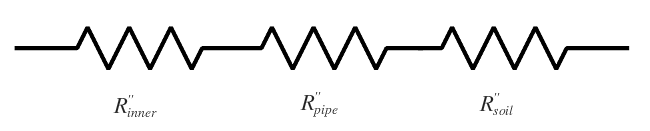
\includegraphics[width=6in]{pictures/Thermal_Resistors.png}
    \caption{Thermal resistor system, moving from the inside fluid convection, conduction through the pipe wall, and conduction to the outside soil.}
\end{figure}
%
\noindent
First we are interested to calculating the internal convection due to the water and the inner pipe surface. First we calculate the Reynolds number for the flow using our estimated volumetric flowrate, inner diameter and cross section of the pipe.
%
\begin{equation}
    { Re }_{ D }=\frac { Q{ D }_{ h } }{ \nu { A }_{ c } } 
\end{equation}
%
Once the Reynolds number is known we can select the correct formulas to calculate the convection coefficient for the pipe. To do this we must first calculate the Nusselt number and combine this with the definition of the average convection coefficient.
%
\begin{equation}
    { N }u_{ D }=\frac { \left( f/8 \right) \left( { Re }_{ D }-1000 \right) Pr }{ 1+12.7(f/8)^{ 1/2 }\left( { Pr }^{ 2/3 }-1 \right)  } 
\end{equation}
%
\begin{equation}
    { N }u_{ D }=\frac { h{ D }_{ h } }{ k } \rightarrow h=\frac { { N }u_{ D }{k}_{water} }{ { D }_{ h } } 
\end{equation}
%
To find the Nusselt number the Gnielinski correlation can be used for flows that has ${ Re }_{ D } > 3000$. The benefit of using this correlation is that it takes into account the roughness of the pipe wall with the Darcy friction factor $f$. The Darcy friction factor can be found using the moody diagram or by using the use of the Colebrook-White equation.
%
\begin{equation}
    f = \frac{64}{Re}\ for\ Re < 2000
\end{equation}
\begin{equation}
    \frac { 1 }{ \sqrt { f }  } =-2\log _{ 10 } \left( \frac { \varepsilon  }{ 3.7D_{ h } } +\frac { 2.51 }{ { Re }\sqrt { f }  }  \right)\ for\ Re \geq 2000
\end{equation}
%
When the flow is not laminar a constant can be used to approximate what the Nusselt number. Using Table 8.1 from \cite{bergman2011fundamentals} the Nusselt number is ${ N }u_{ D }=3.66$. Using this friction factor and Nusselt number equation we can finally find the convection coefficient of the inside pipe. Next the thermal resistance for the pipe wall can be calculated. Using the CES material selector \cite{ces} the following material properties where found for the three common types of pipes used for installation.
%
\begin{table}[H]
\centering
\begin{tabular}{lll}
Type       & Thermal Conductivity (W/mk) & Density (kg/$m^3$) \\ \hline
HDPE Pipe  & 0.461-0.502                 & 947-955                          \\
PVC Pipe   & 0.147-0.209                 & 1300-1490                        \\
CPVC Pipe  & 0.133-0.144                 & 1450-1560                       
\end{tabular}
\end{table}
%
\noindent
Using these conduction values the heat transfer through the pipe can be calculated. Furthermore the heat transfer into the soil can also be calculated in a similar way. We look to find the conduction coefficient of the soil that that geothermal heat pump pipes will be buried in. This will vary from region to region but also it is a function of multiple variables. As seen in the work done by Farouki \cite{farouki1981thermal} the thermal properties vary largely as a function of Quartz content, crushed or natural, coarse or fine, dry density, and degree of saturation. %
\begin{equation}
    { R }_{ total }={ R }_{ inner }+{ R }_{ pipe }+{ R }_{ soil }=\frac { 1 }{ h{ A }_{ s } } +\frac { ln({ { r }_{ o } }/{ { r }_{ i } }) }{ { 2\pi Lk }_{ pipe } } +\frac { ln({ { r }_{ \infty  } }/{ { r }_{ o } }) }{ { 2\pi Lk }_{ soil } } 
\end{equation}
%
We will assume that the user knows this value has has calculated it using the equations noted in \cite{farouki1981thermal}. From this the total resistance can be calculated for the entire system. Now that we know how to calculate the total resistance we can find the outlet temperature by using the log mean temperature difference energy balance. This balances the mass flowrate with the overall change in temperature through the system.
%
\begin{equation}
    \frac { ({ T }_{ \infty  }-{ T }_{ m,o }) }{ ({ T }_{ \infty  }-{ T }_{ m,i }) } =exp\left[ -\frac { 1 }{ \dot { m } { C }_{ p }{ R }_{ tot } }  \right] 
\end{equation}
%
We know what our ${ T }_{ \infty }$, ${ T }_{ m,i }$, pipe type, length, and how to find the total resistance for the material. With these we can calculate the outlet temperature and the total energy transferred into the ground. Both of these values can be used to correctly size a pipe system.